\documentclass[11pt,a4paper]{article}

% ── Idioma y codificacion ─────────────────────────────────────────────
\usepackage[utf8]{inputenc}
\usepackage[T1]{fontenc}
\usepackage[spanish]{babel}

% ── Layout y tipografia ──────────────────────────────────────────────
\usepackage[margin=2.5cm]{geometry}
\usepackage{microtype}
\usepackage{parskip}
\usepackage{setspace}
\onehalfspacing

% ── Tablas y figuras ─────────────────────────────────────────────────
\usepackage{booktabs}
\usepackage{tabularx}
\usepackage{longtable}
\usepackage{multirow}
\usepackage[table]{xcolor}
\usepackage{colortbl}
\usepackage{graphicx}
\usepackage{float}

% ── Listas compactas ─────────────────────────────────────────────────
\usepackage{enumitem}
\setlist[itemize]{nosep, leftmargin=*, topsep=2pt, partopsep=0pt}
\setlist[enumerate]{nosep, leftmargin=*, topsep=2pt, partopsep=0pt}

% ── Cajas y destacados ──────────────────────────────────────────────
\usepackage[most]{tcolorbox}

% ── Headers y footers ────────────────────────────────────────────────
\usepackage{fancyhdr}
\pagestyle{fancy}
\fancyhf{}
\fancyhead[L]{\small Introducci\'{o}n a la Ciencia de Datos 2026}
\fancyhead[R]{\small Tarea 1}
\fancyfoot[C]{\thepage}
\renewcommand{\headrulewidth}{0.4pt}

% ── Links ────────────────────────────────────────────────────────────
\usepackage[colorlinks=true, linkcolor=blue!70!black, urlcolor=blue!70!black, citecolor=blue!70!black]{hyperref}

% ── Penalizaciones para viudas y huerfanas ───────────────────────────
\widowpenalty=10000
\clubpenalty=10000

% ── Colores personalizados ───────────────────────────────────────────
\definecolor{udelar}{RGB}{0, 75, 135}
\definecolor{lightgray}{RGB}{245, 245, 245}
\definecolor{codebg}{RGB}{248, 248, 248}

% ── Codigo monoespaciado ─────────────────────────────────────────────
\usepackage{listings}
\lstset{
    basicstyle=\ttfamily\footnotesize,
    backgroundcolor=\color{codebg},
    frame=single,
    framerule=0pt,
    breaklines=true,
    breakatwhitespace=true,
    columns=fullflexible,
    keepspaces=true,
    xleftmargin=8pt,
    xrightmargin=8pt,
}

% ══════════════════════════════════════════════════════════════════════
\begin{document}

% ── CARATULA ─────────────────────────────────────────────────────────
\begin{titlepage}
\centering
\vspace*{1cm}


\includegraphics[width=0.8\textwidth]{Logo_Fing+Udelar_horizontal_RGB.png}\\
\vspace{1cm}

{\Huge\bfseries Tarea 1 \par}
\vspace{0.5cm}
{\Large\bfseries Introducci\'{o}n a la Ciencia de Datos \par}
\vspace{0.5cm}
{\Large\bfseries Edici\'{o}n 2026 \par}

\vfill

\begin{flushleft}
\large
\textbf{Integrantes:}
\vspace{0.3cm}
\begin{itemize}[label={}, left=0pt]
    \item Tom\'{a}s Alejo Spoturno Gonzalez, 5.165.789-6
    \item Nicol\'{a}s Buero, 5.000.105-4
\end{itemize}
\end{flushleft}

\vfill

\textbf{Universidad de la Rep\'{u}blica}\\
\textbf{Facultad de Ingenier\'{\i}a}\\
\vspace{1cm}
Mayo 2026

\end{titlepage}

% ── INDICE ───────────────────────────────────────────────────────────
\newpage
\tableofcontents
\newpage

% ══════════════════════════════════════════════════════════════════════
% INTRODUCCION
% ══════════════════════════════════════════════════════════════════════
\section{Introducci\'{o}n}

Este informe documenta la resoluci\'{o}n de la Tarea~1 del curso \textit{Introducci\'{o}n a la Ciencia de Datos} (edici\'{o}n 2026). El trabajo se realiza sobre un subconjunto muestreado del dataset abierto \textit{All the News 2.1 -- Component One}, que contiene art\'{\i}culos de noticias publicados en distintos medios de prensa. El objetivo de esta primera entrega es \textbf{cargar, explorar y limpiar} los datos, con vistas a una futura tarea de clasificaci\'{o}n autom\'{a}tica de textos por medio de prensa.

El c\'{o}digo se encuentra en el notebook \texttt{Tarea\_1/2026\_template\_tarea1.ipynb} del repositorio. En este informe se reportan los resultados y las decisiones tomadas; las visualizaciones y tablas se reproducen a partir del notebook ejecutado.

% ══════════════════════════════════════════════════════════════════════
% PARTE 1
% ══════════════════════════════════════════════════════════════════════
\section{Parte 1: Cargado y Limpieza de Datos}

\subsection{A. Exploraci\'{o}n de datos y selecci\'{o}n de los 5 medios principales}

\subsubsection*{Composici\'{o}n del DataFrame}

El DataFrame cargado contiene 30.213 art\'{\i}culos y 12 columnas. Las columnas son: \texttt{idx}, \texttt{article\_idx}, \texttt{date}, \texttt{year}, \texttt{month}, \texttt{day}, \texttt{author}, \texttt{title}, \texttt{article}, \texttt{url}, \texttt{section}, \texttt{publication}. Cada fila representa un art\'{\i}culo de noticias, con metadatos (\texttt{publication}, \texttt{author}, \texttt{date}, \texttt{section}, \texttt{url}) y el contenido textual (\texttt{title}, \texttt{article}).

\subsubsection*{Datos faltantes por columna}

Se evalu\'{o} la cantidad de valores nulos en cada columna. La Tabla~\ref{tab:missing} resume las columnas con datos faltantes.

\begin{table}[H]
\centering
\caption{Columnas con datos faltantes en el DataFrame.}
\label{tab:missing}
\begin{tabular}{l r r}
\toprule
\textbf{Columna} & \textbf{Faltantes} & \textbf{\%} \\
\midrule
\texttt{author} & 11.405 & 37.75\% \\
\texttt{section} & 10.232 & 33.87\% \\
\texttt{article} & 1.176 & 3.89\% \\
\texttt{url} & 141 & 0.47\% \\
\texttt{publication} & 141 & 0.47\% \\
\bottomrule
\end{tabular}
\end{table}

Las columnas con datos faltantes m\'{a}s significativos son \texttt{section} y \texttt{author}: ambas tienen una proporci\'{o}n alta de valores nulos. \texttt{section} no est\'{a} disponible para todos los medios (por ejemplo, \textit{The Hill} no la reporta), y \texttt{author} puede faltar en cables de agencia o en notas sin firma. El resto de los campos cr\'{\i}ticos (\texttt{publication}, \texttt{date}, \texttt{title}, \texttt{article}) est\'{a}n pr\'{a}cticamente completos.

\subsubsection*{Otros problemas de calidad}

Adem\'{a}s de los faltantes, se identificaron los siguientes problemas mediante chequeos manuales:

\begin{itemize}
    \item \textbf{Redundancia entre \texttt{idx} y \texttt{article\_idx}}: la diferencia entre ambas columnas es cero en todas las filas, es decir, contienen exactamente el mismo valor en cada registro. Una de las dos es redundante.
    \item \textbf{Formato heterog\'{e}neo en \texttt{date}}: conviven los formatos \texttt{YYYY-MM-DD} y \texttt{YYYY-MM-DD HH:MM:SS} en distintas filas. Esto obliga a usar \texttt{format='mixed'} al parsear.
    \item \textbf{Tipo de \texttt{month}}: la columna \texttt{month} se almacena como cadena de texto (\texttt{str}), no como entero, a pesar de contener \'{u}nicamente valores num\'{e}ricos del 1 al 12. Lo mismo ocurre con \texttt{year} y \texttt{day}. Conviene convertirlas a entero si se las quisiera utilizar para operaciones num\'{e}ricas, aunque como se discute m\'{a}s abajo son redundantes con \texttt{date}.
    \item \textbf{Redundancia entre \texttt{date} y \texttt{year}, \texttt{month}, \texttt{day}}: las tres \'{u}ltimas son derivables exactamente de \texttt{date}. Se verific\'{o} consistencia (a\~{n}o, mes y d\'{\i}a coinciden con el \texttt{date} parseado en todos los registros donde ambos existen). Por lo tanto pueden eliminarse sin p\'{e}rdida de informaci\'{o}n.
    \item \textbf{URLs}: de las 30.072 URLs presentes, las 30.072 son v\'alidas seg\'un un chequeo regex (esquema \texttt{http}/\texttt{https} y caracteres v\'alidos). No se encontraron URLs con formato inv\'{a}lido en el corpus.
\end{itemize}

\subsubsection*{Selecci\'{o}n de los 5 medios principales}

El dataset contiene art\'{\i}culos de 26 medios de prensa, con una distribuci\'{o}n muy desbalanceada. Para el resto del an\'{a}lisis se trabaja con los \textbf{cinco medios con mayor cantidad de art\'{\i}culos}, cuyos conteos se muestran en la Tabla~\ref{tab:top5}.

\begin{table}[H]
\centering
\caption{Top 5 medios con mayor cantidad de art\'iculos en el dataset.}
\label{tab:top5}
\begin{tabular}{l r r}
\toprule
\textbf{Medio} & \textbf{Art\'iculos} & \textbf{\% del total} \\
\midrule
Reuters & 9.431 & 31.2\% \\
The New York Times & 2.840 & 9.4\% \\
CNBC & 2.623 & 8.7\% \\
The Hill & 2.349 & 7.8\% \\
People & 1.528 & 5.1\% \\
\midrule
\textbf{Total top 5} & \textbf{18.771} & \textbf{62.1\%} \\
\bottomrule
\end{tabular}
\end{table}

A partir de este punto, todos los an\'{a}lisis se realizan sobre el sub-DataFrame \texttt{df\_top\_5}, que contiene 18.771 art\'{\i}culos.


\subsection{B. Visualizaci\'{o}n temporal}

Para visualizar la actividad de los cinco medios a lo largo del tiempo, se gener\'{o} primero una serie por mes y otra por a\~{n}o (ver Figura~\ref{fig:temporal}).

\begin{figure}[H]
\centering
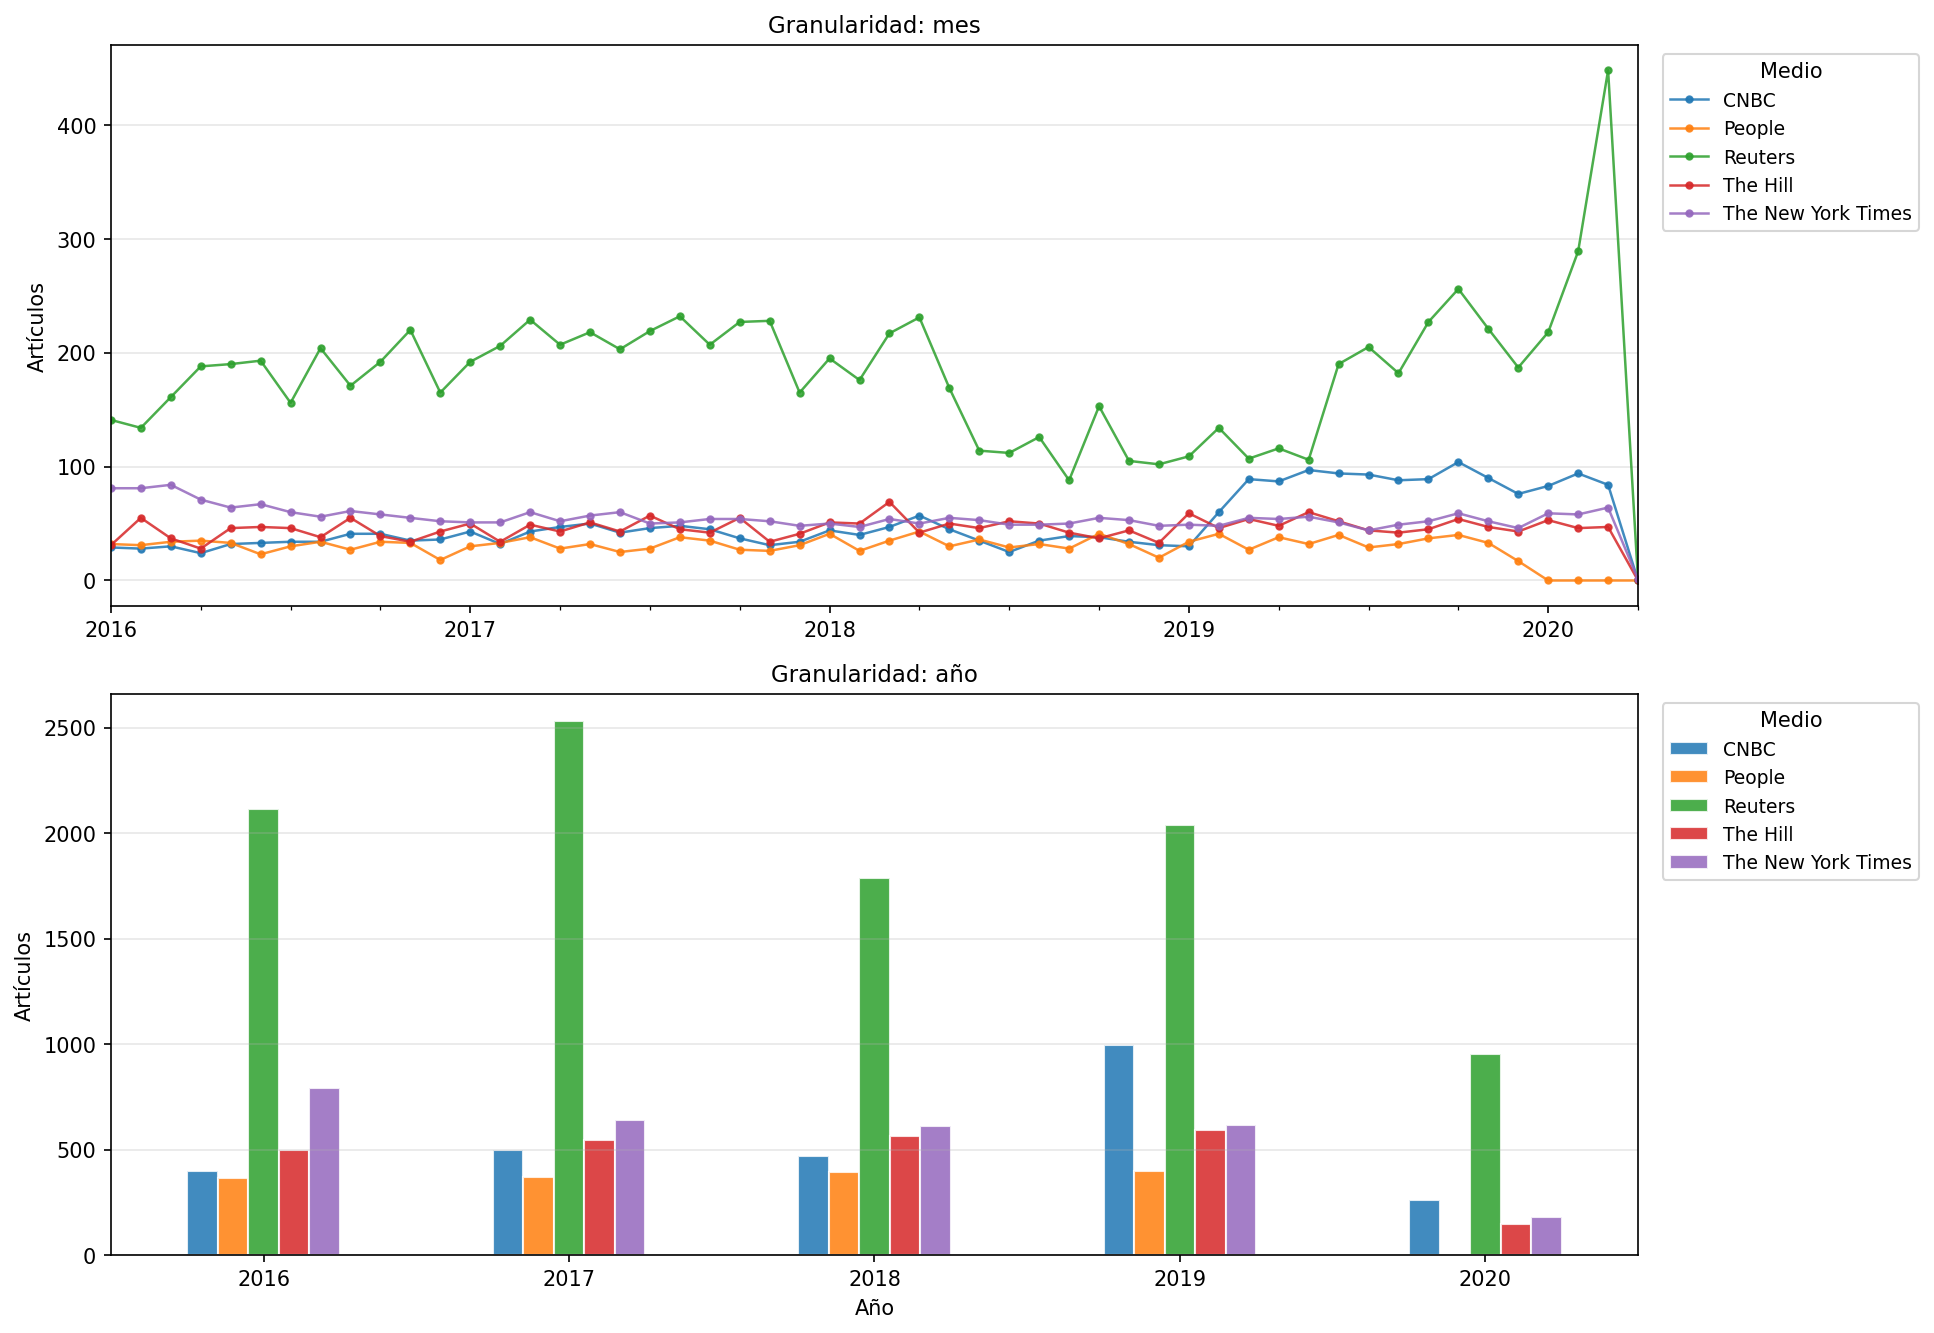
\includegraphics[width=0.95\textwidth]{chart_temporal.png}
\caption{Cantidad de art\'{\i}culos publicados por los 5 medios a lo largo del tiempo (granularidad mes y a\~{n}o).}
\label{fig:temporal}
\end{figure}

\textbf{Observaciones generales.} Los cinco medios cubren aproximadamente el mismo per\'{\i}odo (de 2016-01-01 a 2020-04-01), aunque con vol\'{u}menes muy distintos. \textit{Reuters} domina ampliamente en cantidad de art\'{\i}culos publicados por mes, con un nivel varias veces superior al resto. Le siguen, en un escal\'{o}n intermedio similar entre s\'{\i}, \textit{NYT}, \textit{CNBC} y \textit{The Hill}; \textit{People} aparece como el medio con menor volumen mensual. La cobertura es relativamente uniforme a lo largo de los a\~{n}os, sin saltos abruptos que sugieran cortes en la ingesta del dataset, m\'{a}s all\'{a} de la ca\'{\i}da natural en el extremo derecho de la serie por el corte en abril de 2020 (el dataset finaliza ese mes y por eso 2020 muestra menos art\'{\i}culos acumulados que los a\~{n}os completos previos).

Para detectar patrones c\'{\i}clicos m\'{a}s finos, se calcul\'{o} el promedio de art\'{\i}culos por d\'{\i}a de la semana y por mes del a\~{n}o (Figura~\ref{fig:ciclico}).

\begin{figure}[H]
\centering
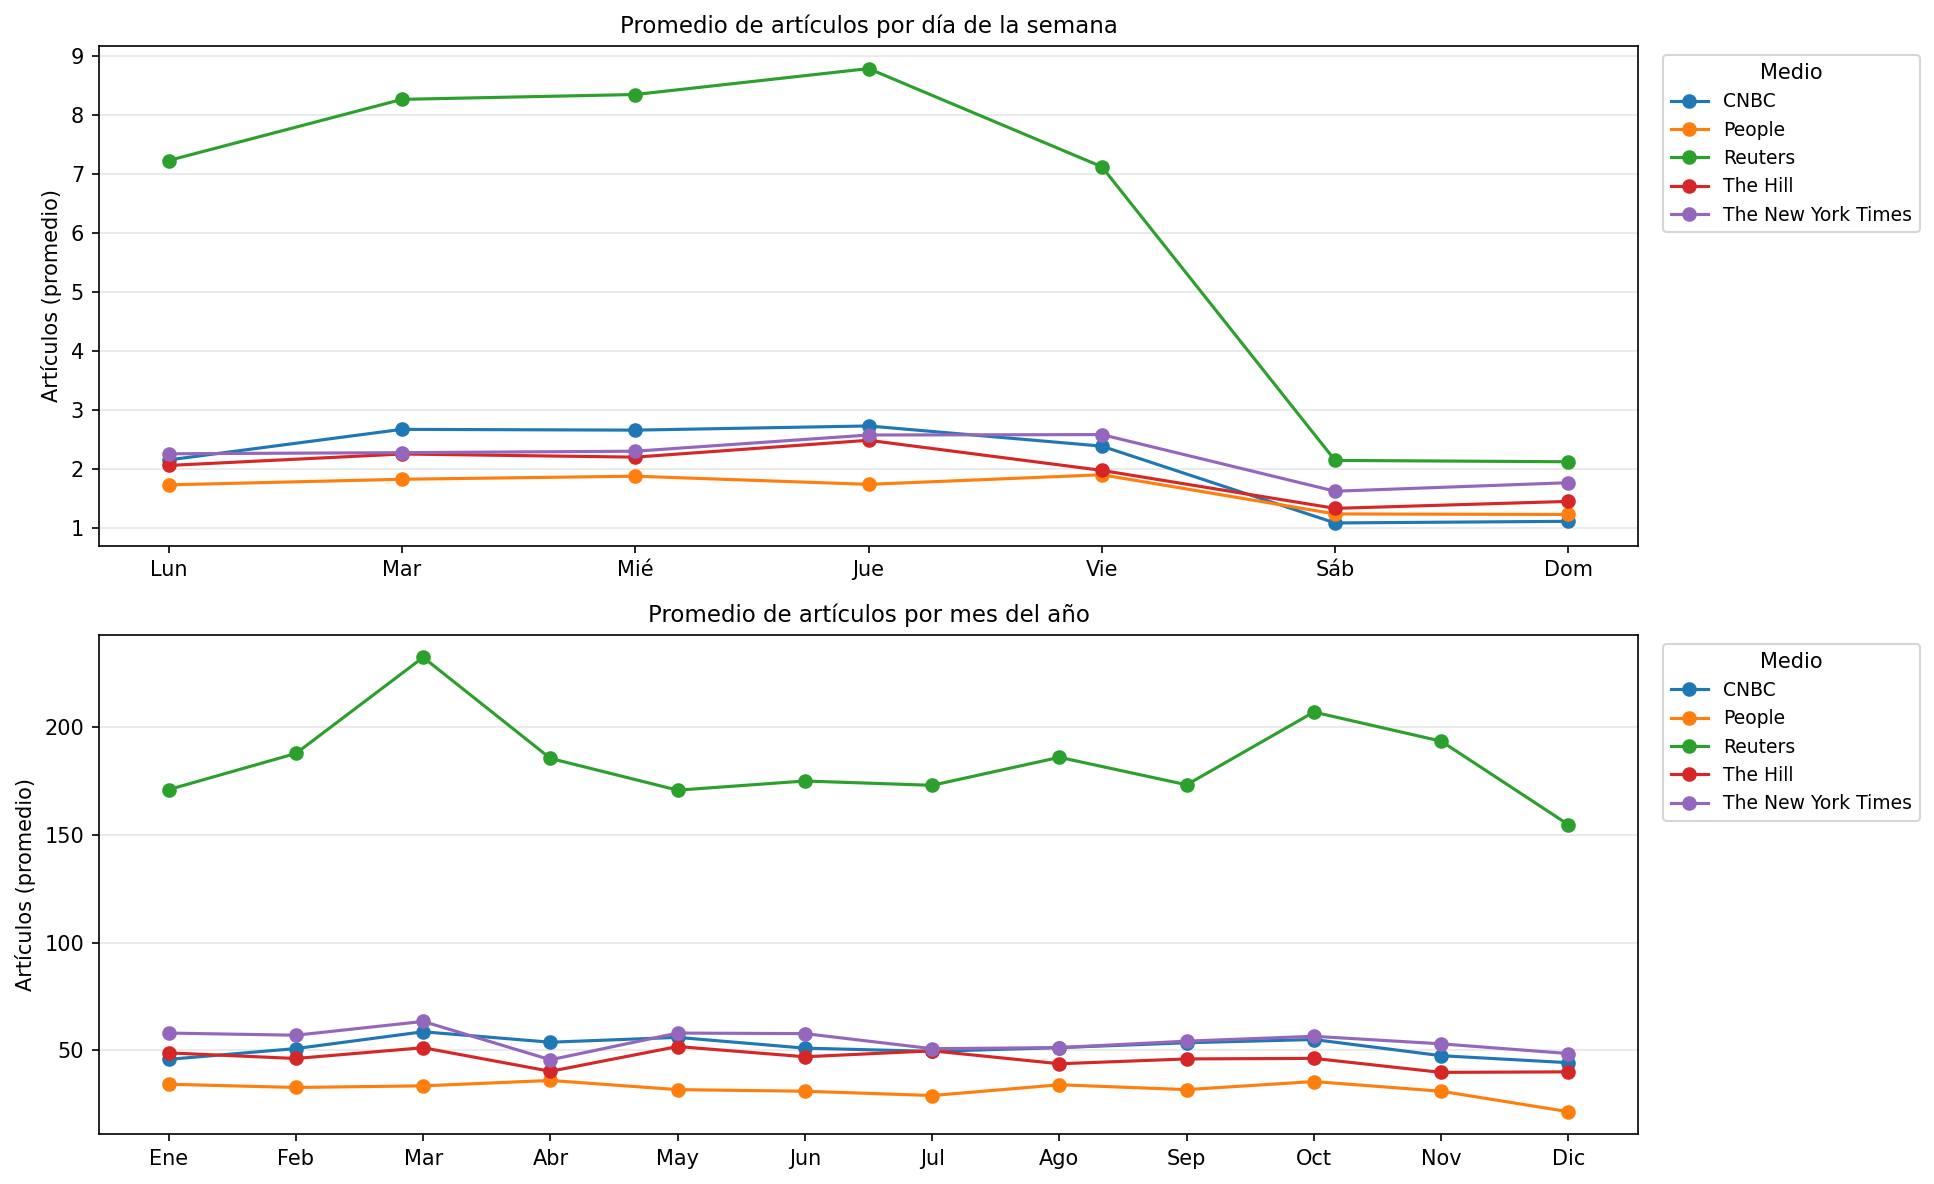
\includegraphics[width=0.95\textwidth]{chart_ciclico.png}
\caption{Promedio de art\'{\i}culos por d\'{\i}a de la semana y por mes del a\~{n}o.}
\label{fig:ciclico}
\end{figure}

\textbf{Patrones c\'{\i}clicos.}
\begin{itemize}
    \item En los \textbf{d\'{\i}as de la semana} se observa una ca\'{\i}da clara los s\'{a}bados y domingos en los medios de tipo agencia y pol\'{\i}tica (\textit{Reuters}, \textit{The Hill}, \textit{CNBC}, \textit{NYT}). \textit{People}, en cambio, mantiene un volumen m\'{a}s parejo, consistente con un perfil editorial de entretenimiento que no depende de la agenda institucional de la semana laboral.
    \item Por \textbf{mes del a\~{n}o} no hay un patr\'{o}n estacional tan marcado: los medios cubren noticias de forma continua durante todo el a\~{n}o.
\end{itemize}

No se realiz\'{o} ning\'{u}n test estad\'{\i}stico; los comentarios se basan exclusivamente en la inspecci\'{o}n visual de las gr\'{a}ficas.


\subsection{C. Limpieza de texto: \texttt{clean\_text}}

Se complet\'{o} la funci\'{o}n \texttt{clean\_text(...)} provista en el notebook con varias transformaciones adicionales. La versi\'{o}n final aplica los siguientes pasos en este orden:

\begin{lstlisting}[language=Python]
def clean_text(df, column_name):
    # 1. Eliminar la primera linea (suele contener titulo/header repetido).
    result = df[column_name].str.replace(r"^[^\n]*\n", "", regex=True)
    # 2. Pasar todo a minusculas.
    result = result.str.lower()
    # 3. Eliminar URLs (http/https): no aportan informacion lexica.
    result = result.str.replace(r'https?://\S+', ' ', regex=True)
    # 4. Eliminar todos los signos de puntuacion / caracteres no alfanumericos.
    #    [^\w\s] captura . ! ; ( ) [ ] { } " ' - _ / | < > # @ % & * + = ^ ~ `
    #    Se reemplaza por espacio para evitar que dos palabras queden pegadas.
    result = result.str.replace(r'[^\w\s]', ' ', regex=True)
    # 5. Eliminar numeros aislados (fechas, cifras, porcentajes).
    result = result.str.replace(r'\b\d+\b', ' ', regex=True)
    # 6. Normalizar saltos de linea y tabulaciones a espacios.
    result = result.str.replace(r'[\n\r\t]', ' ', regex=True)
    # 7. Colapsar multiples espacios consecutivos en uno solo.
    result = result.str.replace(r'\s+', ' ', regex=True)
    # 8. Eliminar espacios al inicio y al final.
    result = result.str.strip()
    return result
\end{lstlisting}

\textbf{Justificaci\'{o}n de cada transformaci\'{o}n agregada respecto a la versi\'{o}n base:}

\begin{itemize}
    \item \textbf{Min\'{u}sculas}: evita que secuencias como \textit{``President''} y \textit{``president''} se cuenten como palabras distintas. Es la transformaci\'{o}n m\'{\i}nima est\'{a}ndar para conteo de palabras.
    \item \textbf{Eliminar URLs}: en notas de prensa aparecen enlaces que no aportan informaci\'{o}n l\'{e}xica para clasificar el medio (y pueden inflar el vocabulario con tokens raros).
    \item \textbf{Reemplazo por espacio en lugar de borrado al eliminar puntuaci\'{o}n}: si se borra el guion o la barra sin reemplazarlo por espacio, dos palabras separadas por ``\texttt{-}'' o ``\texttt{/}'' quedar\'{\i}an pegadas como una sola.
    \item \textbf{Eliminar n\'{u}meros aislados}: fechas, cifras y porcentajes no ayudan a discriminar el estilo editorial de cada medio (son ruido sem\'{a}ntico para esta tarea).
    \item \textbf{Patr\'{o}n regex generalizado}: el c\'{o}digo de base ten\'{\i}a un bucle que cubr\'{\i}a solo cinco s\'{\i}mbolos. Se reemplaz\'{o} por un \'{u}nico patr\'{o}n que captura todos los caracteres que no son alfanum\'{e}ricos ni espacios. Eso elimina en un solo paso toda la puntuaci\'{o}n usual (puntos, comas, signos de pregunta y exclamaci\'{o}n, par\'{e}ntesis, corchetes, llaves, comillas, guiones, barras, etc.) sin tener que enumerarlas a mano.
    \item \textbf{Colapsar espacios m\'{u}ltiples y \texttt{strip()}}: los pasos anteriores generan muchos espacios consecutivos; este paso final normaliza el resultado.
\end{itemize}

Verificaci\'{o}n: se compar\'{o} el texto original contra el texto limpio en una muestra de art\'{\i}culos. Las cadenas resultantes consisten exclusivamente en secuencias de palabras alfanum\'{e}ricas en min\'{u}scula separadas por un \'{u}nico espacio.


\subsection{D. Elecci\'{o}n del campo de texto a utilizar}

Se eligi\'{o} trabajar con el \textbf{cuerpo del art\'{\i}culo} (\texttt{article}).

El objetivo a futuro es construir un perfil de palabras que permita distinguir un medio de otro. Para eso, el volumen de texto importa: los t\'{\i}tulos tienen en promedio del orden de 10 palabras (entre 9.0 y 11.8 palabras por t\'itulo seg\'un el medio), lo que genera perfiles de frecuencia muy ruidosos y dependientes del tema puntual de cada nota. El cuerpo del art\'{\i}culo, en cambio, tiene varios cientos de palabras por art\'{\i}culo en todos los medios, lo que da mucha m\'{a}s se\~{n}al para caracterizar el estilo editorial real.

La Tabla~\ref{tab:lenfields} resume el largo promedio de t\'{\i}tulo y cuerpo por medio.

\begin{table}[H]
\centering
\caption{Largo promedio del t\'itulo y del cuerpo del art\'iculo (en palabras) por medio.}
\label{tab:lenfields}
\begin{tabular}{l r r r}
\toprule
\textbf{Medio} & \textbf{T\'itulo (media)} & \textbf{Cuerpo (media)} & \textbf{Cuerpo (mediana)} \\
\midrule
Reuters & 9.9 & 281.7 & 209.0 \\
The New York Times & 9.0 & 905.8 & 848.5 \\
CNBC & 10.6 & 461.0 & 405.0 \\
The Hill & 11.8 & 572.0 & 464.0 \\
People & 9.7 & 419.0 & 371.0 \\
\bottomrule
\end{tabular}
\end{table}

Adem\'{a}s, el cuerpo captura cosas que el t\'{\i}tulo no: vocabulario t\'{e}cnico, estructura de los p\'{a}rrafos, referencias cruzadas, plantillas editoriales, etc. \textbf{Combinar ambos campos} (t\'{\i}tulo + cuerpo) no aporta demasiado, porque el art\'{\i}culo en general ya contiene toda la informaci\'{o}n del t\'{\i}tulo (y porque el peso relativo del t\'{\i}tulo es despreciable frente al del cuerpo).


\subsection{E. Pistas que identifican al medio de prensa}

Una preocupaci\'{o}n importante para una futura tarea de clasificaci\'{o}n por medio es la presencia de \textbf{marcas en el texto que delaten al medio de manera directa}, sin requerir analizar el estilo editorial. Si esas marcas existen, una clasificadora puede ``hacer trampa'' aprendiendo a detectar la marca en lugar de aprender el estilo.

Revisando manualmente una muestra aleatoria de art\'{\i}culos por medio y luego cuantificando con expresiones regulares sobre todo el corpus, se identificaron las siguientes pistas:

\subsubsection*{Reuters}
\begin{itemize}
    \item \textbf{Dateline al inicio del cuerpo}: el 91.9\% de los art\'{\i}culos contiene la marca \texttt{CIUDAD (Reuters) -} en el cuerpo. Es la firma m\'{a}s reconocible de la agencia.
    \item \textbf{Firma de cierre}: el 56.1\% termina con \texttt{Reporting by X; Editing by Y}.
    \item \textbf{Plantilla de \textit{Further company coverage}}: aparece al final en el 24.2\% de los art\'{\i}culos.
\end{itemize}
Son tres marcas acumuladas que identifican a \textit{Reuters} de forma casi inequ\'{\i}voca.

\subsubsection*{The Hill}
\begin{itemize}
    \item \textbf{Sufijo en el t\'{\i}tulo}: el 100.0\% de los t\'{\i}tulos termina con ``\texttt{| TheHill}''. Es una marca 100\%-sistem\'{a}tica.
    \item \textbf{Footer legal}: el 99.4\% de los art\'{\i}culos termina con el mismo footer (\texttt{Capitol Hill Publishing Corp.} con direcci\'{o}n, tel\'{e}fonos y copyright).
    \item \textbf{URL \texttt{thehill.com} en cuerpo}: marginal pero presente.
    \item \textbf{Artefacto de scraping}: en algunos art\'{\i}culos los nombres de pol\'{\i}ticos quedan duplicados (\textit{John McCainJohn Sidney McCain}), por una superposici\'{o}n del tag de link con el texto.
\end{itemize}

\subsubsection*{CNBC}
\begin{itemize}
    \item \textbf{Cables de Reuters republicados}: el 24.3\% de los art\'{\i}culos de \textit{CNBC} tiene el dateline \texttt{(Reuters)} y/o la firma \texttt{Reporting by}, porque \textit{CNBC} republica cables de la agencia.
    \item \textbf{Auto-menci\'{o}n}: el 34.8\% menciona ``CNBC'' en el cuerpo.
    \item \textbf{Footer Mad Money}: bloque recurrente que termina con \texttt{madcap@cnbc.com}.
\end{itemize}
No hay un boilerplate tan uniforme como en \textit{Reuters} o \textit{The Hill} para el contenido original.

\subsubsection*{The New York Times}
\begin{itemize}
    \item \textbf{Auto-menci\'{o}n}: el 18.9\% menciona ``New York Times''.
    \item \textbf{URL \texttt{nytimes.com}}: presente en una fracci\'{o}n menor.
    \item \textbf{Footers por secci\'{o}n}: a diferencia de los otros medios, las pistas no son un \'{u}nico boilerplate sino \textit{footers espec\'{\i}ficos por secci\'{o}n}: art\'{\i}culos de \textit{Opinion} terminan con \texttt{@NYTopinion}, los de \textit{Learning Network} con \textit{``Learning Network staff''}, y los de \textit{NY Today} con \textit{``New York Today''}. Cada uno representa un porcentaje peque\~{n}o, pero todos son se\~{n}ales directas del medio.
\end{itemize}

\subsubsection*{People}
\begin{itemize}
    \item \textbf{Convenci\'{o}n editorial \texttt{tells/told PEOPLE}}: el 28.4\% usa esta f\'{o}rmula para atribuir citas, que es propia de la revista.
    \item \textbf{Auto-menci\'{o}n en may\'{u}sculas}: el 50.3\% menciona ``PEOPLE'' en may\'{u}sculas.
    \item \textbf{Footer \textit{PEOPLE Now}}: bloque recurrente que promociona el programa de streaming del medio.
    \item \textbf{URL \texttt{people.com}}: muy escaso.
\end{itemize}

\subsubsection*{Verificaci\'{o}n cruzada}

Para confirmar que cada patr\'{o}n es propio de su medio (y no aparece accidentalmente en otros), se hizo una verificaci\'{o}n cruzada. La Tabla~\ref{tab:cross} muestra el porcentaje de art\'{\i}culos de cada medio que contiene cada uno de los patrones identificadores.

\begin{table}[H]
\centering\small
\caption{Porcentaje de art\'iculos de cada medio que contiene cada patr\'on identificador. Los porcentajes altos en la columna del medio de origen y bajos en el resto confirman que el patr\'on identifica al medio.}
\label{tab:cross}
\begin{tabularx}{\textwidth}{X r r r r r}
\toprule
\textbf{Patr\'on} & \textbf{Reuters} & \textbf{The New York Times} & \textbf{CNBC} & \textbf{The Hill} & \textbf{People} \\
\midrule
Reuters dateline (Reuters) & 91.9\% & 0.2\% & 24.3\% & 0.1\% & 0.0\% \\
The Hill | TheHill en título & 0.0\% & 0.0\% & 0.0\% & 100.0\% & 0.0\% \\
The Hill footer Capitol Hill & 0.0\% & 0.0\% & 0.0\% & 99.4\% & 0.0\% \\
CNBC mencionado en cuerpo & 0.3\% & 0.5\% & 34.8\% & 0.6\% & 0.2\% \\
NYT nytimes.com en cuerpo & 0.0\% & 8.4\% & 0.0\% & 0.0\% & 0.0\% \\
People tells/told PEOPLE & 0.0\% & 0.0\% & 0.0\% & 0.0\% & 28.4\% \\
\bottomrule
\end{tabularx}
\end{table}

Como era esperable, los patrones tienen alta concentraci\'{o}n en su medio de origen y baja presencia en los dem\'{a}s; la \'{u}nica excepci\'{o}n notable es el dateline \texttt{(Reuters)} que tambi\'{e}n aparece en \textit{CNBC} por la republicaci\'{o}n de cables.

\subsubsection*{Adem\'{a}s, la columna \texttt{url}}

El dominio de la \texttt{url} identifica al medio al 100\% en todos los casos. Sin embargo, en este trabajo el objetivo es clasificar a partir del \emph{texto} de los art\'{\i}culos, por lo que la columna \texttt{url} no debe usarse como predictor; se la considera \'{u}til \'{u}nicamente como ground-truth (junto con \texttt{publication}).

\subsubsection*{Decisi\'{o}n: eliminar o reducir el impacto de las pistas}

Para una tarea de clasificaci\'{o}n por estilo editorial, \textbf{conviene reducir el impacto de estas marcas}. Las dos opciones consideradas son:

\begin{enumerate}
    \item \textbf{Eliminarlas como plantillas} (regex sobre el texto crudo) antes del conteo de palabras. Esta es la decisi\'{o}n adoptada para la Parte 2 (no documentada en este informe): se definen patrones espec\'{\i}ficos para el dateline de \textit{Reuters}, el footer legal de \textit{The Hill}, el handle \texttt{@NYTopinion} de \textit{NYT}, etc.
    \item \textbf{Eliminar tokens aislados} (\texttt{reuters}, \texttt{cnbc}, \texttt{nytimes}, \texttt{thehill}, \texttt{nyt}, \texttt{people}) cuando aparecen como palabras sueltas tras la tokenizaci\'{o}n.
\end{enumerate}

Las dos opciones se complementan: la primera limpia frases completas (evitando que palabras genuinas como \texttt{capitol} o \texttt{hill} se pierdan por estar dentro de una plantilla), mientras que la segunda atrapa menciones aisladas que se escapan a las regex.


\subsection{F. Restricci\'{o}n por secci\'{o}n tem\'{a}tica o per\'{\i}odo temporal}

\subsubsection*{Restricci\'{o}n por secci\'{o}n tem\'{a}tica}

La idea es interesante en principio: si se comparan art\'{\i}culos del mismo tema, cualquier diferencia en frecuencia de palabras refleja estilo editorial y no simplemente el \textit{topic}. Sin embargo, en este dataset hay dos problemas concretos que la hacen inviable:

\begin{itemize}
    \item \textbf{\textit{The Hill} no tiene la columna \texttt{section}} reportada en ninguno de sus art\'{\i}culos (2349 de 2349 art\'iculos, 100\% sin secci\'on).
    \item \textbf{\textit{People} cubre exclusivamente entretenimiento} (\textit{tv, movies, celebrity, style}) y no tiene art\'{\i}culos de pol\'{\i}tica ni econom\'{\i}a, que son los temas dominantes en los otros cuatro medios. Restringir por una secci\'{o}n com\'{u}n equivaldr\'{\i}a a eliminar \textit{People} del an\'{a}lisis.
\end{itemize}

Adem\'{a}s, conceptualmente, \textbf{el tema que cubre cada medio es parte de su identidad editorial}: \textit{Reuters} es una agencia de cable financiera, \textit{People} es una revista de celebrities. Esa diferencia tem\'{a}tica no es ``ruido'', sino una caracter\'{\i}stica real del medio que una clasificadora puede (y deber\'{\i}a) aprovechar.

La Tabla~\ref{tab:secciones} resume las secciones m\'{a}s frecuentes en cada medio.

\begin{table}[H]
\centering\small
\caption{Secciones m\'as frecuentes por medio (top 5) y proporci\'on de art\'iculos sin secci\'on reportada.}
\label{tab:secciones}
\begin{tabularx}{\textwidth}{l r X}
\toprule
\textbf{Medio} & \textbf{\% sin secci\'on} & \textbf{Top 5 secciones} \\
\midrule
Reuters & 1\% & \textit{World News} (1.227), \textit{Market News} (1.218), \textit{Business News} (1.076), \textit{Financials} (679), \textit{Intel} (465) \\
The New York Times & 2\% & \textit{world} (329), \textit{opinion} (319), \textit{us} (297), \textit{arts} (239), \textit{sports} (235) \\
CNBC & 18\% & \textit{Wires} (733), \textit{Politics} (175), \textit{Tech} (146), \textit{Markets} (64), \textit{Market Insider} (63) \\
The Hill & 100\% & \textbf{sin datos de secci\'on} \\
People & 0\% & \textit{tv} (280), \textit{movies} (153), \textit{style} (136), \textit{crime} (130), \textit{celebrity} (112) \\
\bottomrule
\end{tabularx}
\end{table}

\subsubsection*{Restricci\'{o}n por per\'{\i}odo temporal}

Los cinco medios cubren aproximadamente el mismo per\'{\i}odo (de 2016-01-01 a 2020-04-01), con distribuci\'{o}n bastante uniforme. No hay un argumento fuerte para acotarlo: restringir a un a\~{n}o en particular reducir\'{\i}a el tama\~{n}o de muestra de forma significativa sin eliminar el problema del sesgo tem\'{a}tico, que es la raz\'{o}n principal por la que se evaluar\'{\i}a esta restricci\'{o}n.

\subsubsection*{Decisi\'{o}n}

\textbf{No se aplica ninguna de las dos restricciones} en este trabajo, por las razones expuestas: la restricci\'{o}n por secci\'{o}n elimina informaci\'{o}n leg\'{\i}tima del estilo editorial, y la restricci\'{o}n temporal no aporta una ganancia evidente.

\newpage
\section{Parte 2: Conteo de palabras y visualizaciones}

\subsection*{Preparaci\'{o}n: tokens limpios}

Para los conteos de palabras de esta parte se construye una columna \texttt{Tokens} que parte de \texttt{CleanText} (Parte 1.C) y le aplica dos filtros adicionales:
\begin{itemize}
    \item \textbf{Stopwords en ingl\'{e}s} (lista de NLTK): \textit{the, of, to, and, in, ...}. Son las palabras m\'{a}s frecuentes del idioma y no diferencian un medio de otro, por lo que dominar\'{\i}an cualquier ranking sin aportar informaci\'{o}n.
    \item \textbf{Identificadores del propio medio} detectados en 1.E (\textit{reuters, cnbc, nytimes, nyt, thehill, ...}). Si no se eliminaran, el ranking de palabras frecuentes de cada medio quedar\'{\i}a encabezado por el nombre del propio medio, lo cual es un resultado trivial y oculta las diferencias reales.
\end{itemize}

Adem\'{a}s, antes de tokenizar se remueven mediante regex las plantillas reiteradas (dateline de Reuters, firmas \textit{``Reporting by''} / \textit{``Editing by''}, footer legal de \textit{The Hill}, etc.). Si solo se filtraran las palabras sueltas, palabras leg\'{\i}timas como \textit{capitol} o \textit{hill} se perder\'{\i}an por estar dentro del footer; eliminando la frase completa solo se descarta el boilerplate y se preservan esas palabras cuando aparecen en contextos editoriales reales.

\subsection{A. Palabras m\'{a}s frecuentes por medio}

Se construye un ranking de las palabras m\'{a}s frecuentes para cada uno de los cinco medios. La frecuencia se reporta en t\'{e}rminos \textbf{relativos} (porcentaje sobre el total de tokens del medio), porque los vol\'{u}menes de texto son muy distintos entre medios y los conteos absolutos no son comparables.

Se incluy\'{o} primero una versi\'{o}n \textbf{ingenua} (sobre \texttt{CleanText}, sin filtrar stopwords ni pistas) para evidenciar el problema: los rankings de los cinco medios resultan casi id\'{e}nticos, encabezados siempre por las mismas palabras funcionales del ingl\'{e}s (\textit{the, of, to, and, ...}). El gr\'{a}fico es poco informativo y no permite comparar nada entre medios.

La versi\'{o}n \textbf{filtrada} (sobre \texttt{Tokens}, ya sin stopwords ni identificadores del medio) ya muestra diferencias claras: vocabulario financiero / de cable en Reuters y CNBC, vocabulario pol\'{\i}tico en The Hill, vocabulario m\'{a}s narrativo en NYT, y vocabulario de entretenimiento y celebridades en People. Como complemento se incluye un \textit{heatmap} con las top-10 palabras de cada medio puestas en la misma escala: as\'{\i} se ve, por ejemplo, que \textit{trump} o \textit{house} pesan muy distinto en The Hill que en People.

\paragraph{Ideas para modificar la visualizaci\'{o}n (sin implementar).}
\begin{itemize}
    \item \textbf{Por secci\'{o}n tem\'{a}tica}: rehacer el top-N restringi\'{e}ndose a una misma \texttt{section} (por ejemplo \textit{politics}); lo que aparece son diferencias de estilo dentro del mismo tema y no diferencias de cobertura. Limitaci\'{o}n: \textit{The Hill} no reporta secci\'{o}n y \textit{People} cubre casi solo entretenimiento.
    \item \textbf{Por fecha}: graficar la serie de tiempo (por mes o trimestre) de unas pocas palabras-clave (\textit{trump, biden, covid, election, ...}) por medio, para ver c\'{o}mo reacciona cada medio frente a un mismo evento; o comparar el top-N de un a\~{n}o contra el de otro dentro del mismo medio para detectar cambios de agenda.
    \item \textbf{Por tipo de noticia}: usar \texttt{section} como proxy de tipo (\textit{opinion / business / politics / sports / ...}) y rehacer la visualizaci\'{o}n agrupando por tipo en lugar de por medio.
\end{itemize}

\subsection{B. Medios con mayor cantidad de palabras}

Se cuenta el total de palabras (separadas por espacios sobre \texttt{CleanText}) por medio. La Figura~\ref{fig:2b} muestra dos vistas complementarias.

\begin{figure}[H]
\centering
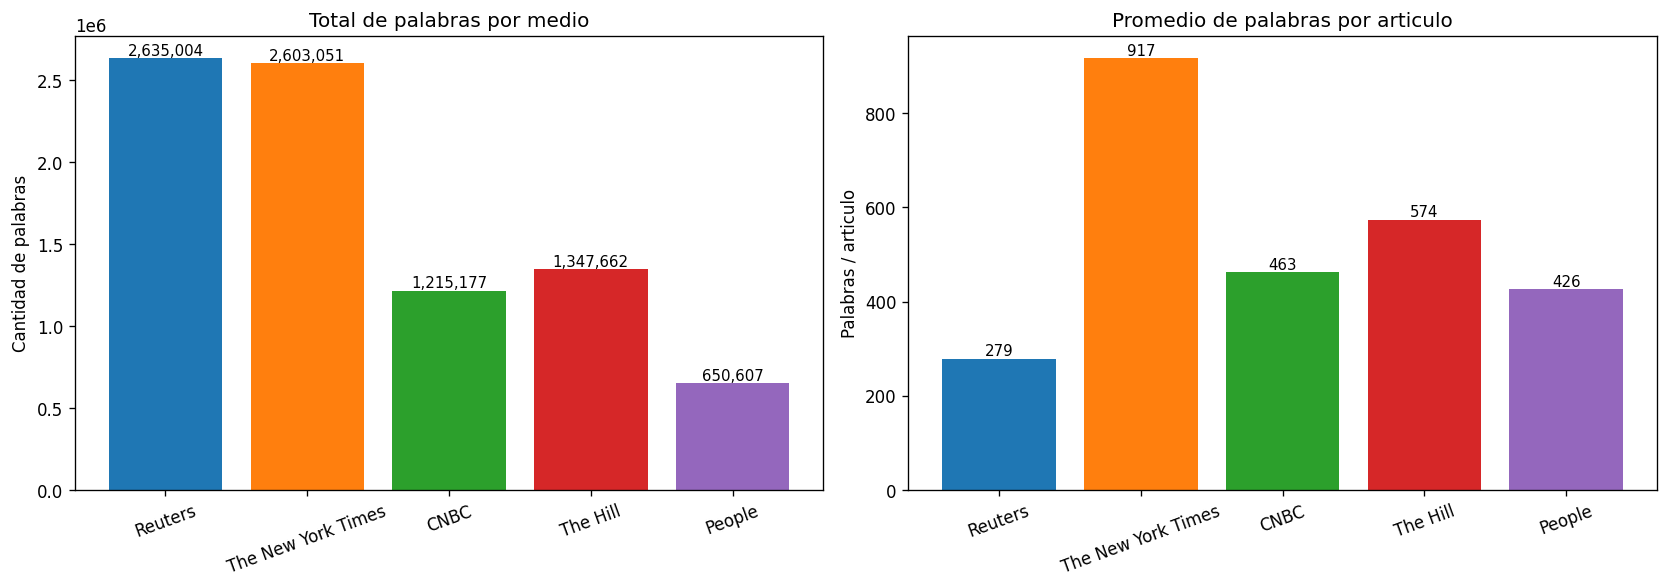
\includegraphics[width=0.95\textwidth]{chart_2b.png}
\caption{Cantidad de palabras por medio. Izquierda: total acumulado. Derecha: promedio por art\'{\i}culo.}
\label{fig:2b}
\end{figure}

\paragraph{Problema observado.} El gr\'{a}fico de la izquierda est\'{a} dominado por \textit{Reuters} y \textit{NYT} con cifras similares (~2,6 millones de palabras cada uno), seguidos a distancia por el resto. Pero esa lectura es enga\~{n}osa: \textit{Reuters} aporta tantas palabras porque tiene \textbf{muchos m\'{a}s art\'{\i}culos} que el resto (9.431 frente a 1.500--2.800 de los otros, ver Tabla~\ref{tab:top5}), no porque sus art\'{\i}culos sean largos. La m\'{e}trica ``total de palabras'' mezcla dos cosas distintas: cantidad de art\'{\i}culos y largo medio por art\'{\i}culo.

\paragraph{Forma de resolverlo.} La m\'{e}trica adecuada para comparar el largo de las notas es el \textbf{promedio de palabras por art\'{\i}culo} (gr\'{a}fico de la derecha). Ah\'{\i} se ve un orden completamente distinto: \textit{NYT} es claramente el medio con notas m\'{a}s largas (917 palabras por art\'{\i}culo en promedio), seguido por \textit{The Hill} (574), \textit{CNBC} (463) y \textit{People} (426), mientras que \textit{Reuters} aparece \'{u}ltimo (279), consistente con su perfil de cable corto. El cambio de orden entre las dos vistas confirma que el total y el promedio responden preguntas distintas.

\subsection{C. Matriz de menciones entre medios}

Se construye una matriz $5 \times 5$ donde la entrada $(i, j)$ cuenta cu\'{a}ntas veces los art\'{\i}culos del medio $i$ mencionan al medio $j$. El conteo se hace sobre el texto original (sin \texttt{clean\_text}) para preservar may\'{u}sculas y poder distinguir, por ejemplo, el nombre propio \textit{``People''} (revista) de la palabra com\'{u}n \textit{``people''}.

Para cada medio se defini\'{o} un patr\'{o}n regex con los nombres con los que aparece mencionado en los textos:
\begin{itemize}
    \item \textit{Reuters}: \texttt{Reuters} (case-insensitive).
    \item \textit{The Hill}: \texttt{The Hill} o \texttt{TheHill}.
    \item \textit{CNBC}: \texttt{CNBC}.
    \item \textit{The New York Times}: \texttt{The New York Times}, \texttt{NYT} o \texttt{nytimes}.
    \item \textit{People}: solo formas estrictas (\texttt{PEOPLE} en may\'{u}sculas, \texttt{People magazine}, \texttt{people.com}). Si se usara \textit{``people''} a secas se confundir\'{\i}a con la palabra com\'{u}n y la columna quedar\'{\i}a inflada artificialmente.
\end{itemize}

La Figura~\ref{fig:2c} muestra el resultado como heatmap. La diagonal (auto-menciones) se enmascara porque las auto-referencias son muy altas (Reuters se menciona a s\'{\i} mismo 11.623 veces) y aportan poco al objetivo de la matriz.

\begin{figure}[H]
\centering
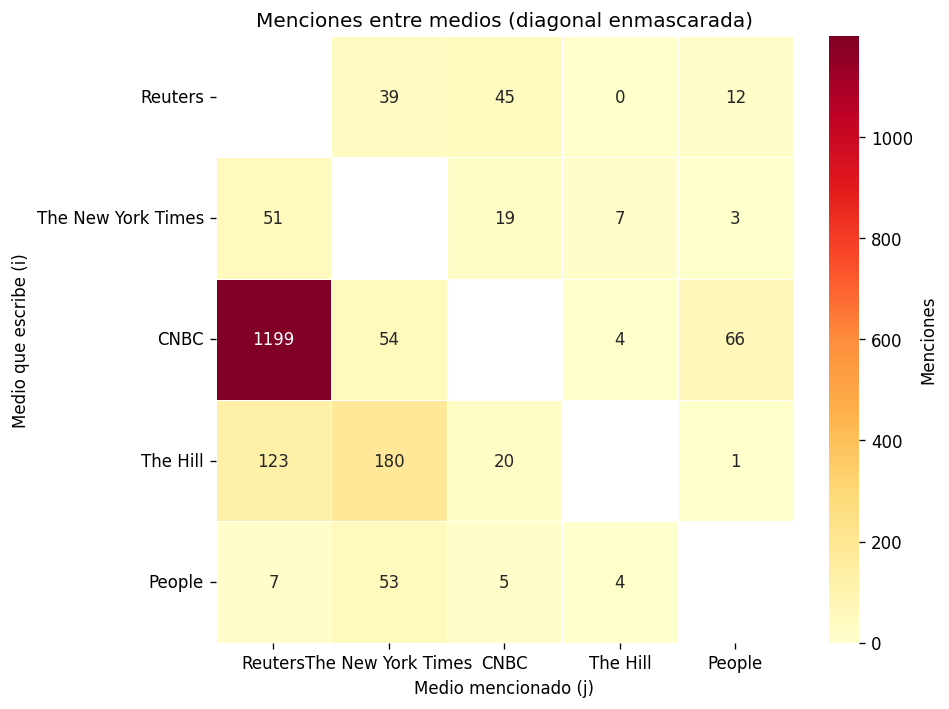
\includegraphics[width=0.7\textwidth]{chart_2c.png}
\caption{Matriz de menciones entre medios. La entrada $(i, j)$ es la cantidad de veces que los art\'{\i}culos del medio $i$ mencionan al medio $j$. Diagonal enmascarada.}
\label{fig:2c}
\end{figure}

\paragraph{Observaciones.}
\begin{itemize}
    \item \textbf{CNBC depende fuertemente de Reuters como fuente}: 1.199 menciones, muy por encima de cualquier otro par. Esto es consistente con lo observado en 1.E, donde un 24\% de los art\'{\i}culos de CNBC inclu\'{\i}an el dateline ``(Reuters)''. CNBC republica cables de Reuters con frecuencia.
    \item \textbf{Las menciones no son sim\'{e}tricas}. \textit{The Hill} menciona a \textit{NYT} 180 veces, pero \textit{NYT} menciona a \textit{The Hill} solo 7 veces. \textit{The Hill} usa al NYT como fuente o referencia mucho m\'{a}s de lo que el NYT habla de \textit{The Hill}. Algo similar pasa con \textit{The Hill} citando a Reuters (123) versus Reuters citando a \textit{The Hill} (0).
    \item \textbf{Reuters apenas menciona al resto}: 39 al NYT, 45 a CNBC, 0 a The Hill, 12 a People. Coherente con su estilo de cable: reporta hechos, no comenta lo que dijeron otros medios.
    \item \textbf{People queda casi aislada en cuanto a menciones recibidas}: salvo CNBC que la menciona 66 veces (probablemente notas de entretenimiento o farandula), los dem\'{a}s la mencionan en cifras de un d\'{\i}gito.
\end{itemize}

\subsection{D. Preguntas propuestas}

A partir de los datos analizados se proponen tres preguntas que podr\'{\i}an explorarse en trabajos posteriores, junto con un camino de an\'{a}lisis sin implementar.

\paragraph{Pregunta 1 -- Largo de los art\'{\i}culos.}
\textit{¿C\'{o}mo se distribuye el largo de los art\'{\i}culos dentro de cada medio? ¿Hay medios con largos muy homog\'{e}neos y otros con mucha varianza?}

\textbf{Camino.} Aprovechando la columna \texttt{NumWords} calculada en 2.B, mirar las distribuciones por medio (mediana, desv\'{\i}o est\'{a}ndar y un boxplot por medio). El promedio mostrado en 2.B esconde la dispersi\'{o}n: un medio podr\'{\i}a tener un promedio similar a otro y aun as\'{\i} alternar entre cables muy cortos y notas muy largas. El boxplot separa ``medio que escribe siempre lo mismo de largo'' de ``medio que mezcla formatos''.

\paragraph{Pregunta 2 -- Reciprocidad de las menciones.}
\textit{¿Las menciones entre medios son rec\'{\i}procas? ¿Cu\'{a}les pares son sim\'{e}tricos y cu\'{a}les muy asim\'{e}tricos?}

\textbf{Camino.} Comparar la matriz \texttt{mentions\_matrix} de 2.C con su traspuesta. Si la entrada $(i, j)$ es muy distinta de $(j, i)$, hay una asimetr\'{\i}a (el medio $i$ depende de $j$ como fuente pero no al rev\'{e}s). Como vimos en las observaciones, ya hay ind\'{\i}cios fuertes (\textit{The Hill} cita a \textit{NYT} 180 veces, \textit{NYT} a \textit{The Hill} solo 7); una inspecci\'{o}n par a par permitir\'{\i}a caracterizar mejor estas relaciones de ``quien usa a quien como fuente''.

\paragraph{Pregunta 3 -- Vocabulario distintivo por medio.}
\textit{M\'{a}s all\'{a} de los identificadores obvios (nombres del propio medio, firmas), ¿cada medio tiene un vocabulario propio que lo diferencia del resto?}

\textbf{Camino.} Partiendo de los \texttt{Tokens} ya filtrados en 2.A, calcular para cada palabra su frecuencia relativa en cada medio y quedarse con las palabras que aparecen mucho en un medio y poco en los otros (alta diferencia entre el m\'{a}ximo y el m\'{\i}nimo de su frecuencia entre los cinco medios). El heatmap de 2.A ya hace una versi\'{o}n inicial de esto sobre el top-N de cada medio; el camino aqu\'{\i} es extenderlo a todo el vocabulario para detectar palabras distintivas que no necesariamente est\'{a}n en el top, pero s\'{\i} son caracter\'{\i}sticas de un \'{u}nico medio.

\end{document}
